\documentclass[titlepage]{article}
\usepackage[utf8]{inputenc}
\usepackage[T1]{fontenc}
\usepackage{listings}
\usepackage{xcolor}
\usepackage{tabularx}
\usepackage{amssymb}
\usepackage{graphicx}
\usepackage{caption}

\title{Rapport MT10 - TP1 : Groupes d’ordre 4}
\author{Martin Schneider, Océane Bordeau}
\date{5 avril 2022}

\setlength{\parindent}{0pt}
\definecolor{codegreen}{rgb}{0,0.6,0}
\definecolor{codegray}{rgb}{0.5,0.5,0.5}
\definecolor{codepurple}{rgb}{0.58,0,0.82}
\definecolor{codeblue}{rgb}{0,0,255}
\definecolor{backcolour}{rgb}{0.95,0.95,0.92}

\lstdefinestyle{mystyle}{ 
    commentstyle=\color{magenta},
    keywordstyle=\color{codeblue},
    numberstyle=\tiny\color{codegray},
    stringstyle=\color{codepurple},
    basicstyle=\ttfamily\footnotesize,
    breakatwhitespace=false,         
    breaklines=true,                 
    captionpos=b,                    
    keepspaces=true,                                  
    showspaces=false,                
    showstringspaces=false,
    showtabs=false,                  
    tabsize=2
}

\lstset{style=mystyle}

\begin{document}
    \maketitle
    \tableofcontents
    \pagebreak
    \textbf{Question 0 :}

    \textbf{\emph{Définition d'un groupe :}} Un groupe est un triplet (G, *, e) où G est un ensemble, * une application
    \[*:G \times G \longrightarrow G\]
    \[(x, x') \longrightarrow x*x'\]
    et $e \in G$ tel que : 

    (i) e est un \textbf{élément neutre} : \[(\forall x \in G) \quad x*e=x \quad et \quad e*x=x\]
    (ii) * est \textbf{associative} : \[(\forall x, x', x'' \in G) \quad (x*x')*x''=x*(x'*x'')\]
    (iii) Tout élément de G adment un \textbf{symetrique} : \[(\forall x \in G)(\exists y \in G) \quad x*y=e \quad et \quad y*x=e\]

    \textbf{\emph{Définition d'un morphisme de groupe :}} Soient (G, *, e) et (G', *', e') deux groupes. 
    Une application de G dans G' est un morphisme de groupe si elle est compatible avec les structures de groupe.
    \[(\forall x, y \in G) \quad f(x*y)=f(x)*'f(y)\]

    \section{Test d'une loi}
        \subsection{Codage d'une loi sur un ensemble}
        \textbf{Question 1 :}

        Groupe $(\mathbb{Z}/4\mathbb{Z}, +, 0)$
        \[E = \{\dot{0}, \dot{1}, \dot{2}, \dot{3}\}\]

        \[t=\begin{tabular}{| c || c | c | c | c |}
            \hline
            $x$\textbackslash $x'$ & $\dot{0}$ & $\dot{1}$ & $\dot{2}$ & $\dot{3}$ \\ \hline \hline
            $\dot{0}$ & $\dot{0}$ & $\dot{1}$ & $\dot{2}$ & $\dot{3}$ \\ \hline
            $\dot{1}$ & $\dot{1}$ & $\dot{2}$ & $\dot{3}$ & $\dot{0}$ \\ \hline
            $\dot{2}$ & $\dot{2}$ & $\dot{3}$ & $\dot{0}$ & $\dot{1}$ \\ \hline
            $\dot{3}$ & $\dot{3}$ & $\dot{0}$ & $\dot{1}$ & $\dot{2}$ \\
            \hline
        \end{tabular}\]

        Groupe $(\mathbb{Z}/2\mathbb{Z} \times \mathbb{Z}/2\mathbb{Z}, +, 0)$
        \[E = \{(0, 0), (1, 0), (0, 1), (1, 1)\}\]
  
        \[t=\begin{tabular}{| c || c | c | c | c |}
            \hline
            $x$\textbackslash $x'$ & (0, 0) & (1, 0) & (0, 1) & (1, 1) \\ \hline \hline
            (0, 0) & (0, 0) & (1, 0) & (0, 1) & (1, 1) \\ \hline
            (1, 0) & (1, 0) & (0, 0) & (1, 1) & (0, 1) \\ \hline
            (0, 1) & (0, 1) & (1, 1) & (0, 0) & (1, 0) \\ \hline
            (1, 1) & (1, 1) & (0, 1) & (1, 0) & (0, 0) \\
            \hline
        \end{tabular}\]

        \textbf{\emph{Avec SageMath}}
        \vspace*{2mm}

        Groupe $(\mathbb{Z}/4\mathbb{Z}, +, 0)$ :
        \vspace*{2mm}

        \begin{tabularx}{11.5cm}{|p{0.60cm}|X|}
            \hline
            \verb|In|
            & 
            \verb|C4 = groups.permutation.Cyclic(4)|
            \\
            \hline
        \end{tabularx}
        
        \begin{tabularx}{11.5cm}{|p{0.60cm}|X|}
            \hline
            \verb|In|
            & 
            \verb|E4 = C4.cayley_table().column_keys()|
            \\
            \hline
        \end{tabularx}

        \begin{tabularx}{11.5cm}{|p{0.60cm}|X|}
            \hline
            \verb|In|
            & 
            \verb|t_C4 = C4.cayley_table().table()|
            \\
            \hline
        \end{tabularx}
        
        \begin{tabularx}{11.5cm}{|p{0.60cm}|X|}
            \hline
            \verb|In|
            & 
            \verb|print(t_C4)|
            \\
            \hline
        \end{tabularx}

        \begin{tabularx}{11.5cm}{|p{0.60cm}|X|}
            \hline
            \verb|Out|
            & 
            {\setlength{\arraycolsep}{2ex}
            \[\begin{array}{r|*{4}{r}}
                \multicolumn{1}{c|}{\ast}&a&b&c&d\\\hline
                {}a&a&b&c&d\\
                {}b&b&c&d&a\\
                {}c&c&d&a&b\\
                {}d&d&a&b&c\\
            \end{array}\]}
            \\
            \hline
        \end{tabularx}

        \vspace*{6mm}
        Groupe $(\mathbb{Z}/2\mathbb{Z} \times \mathbb{Z}/2\mathbb{Z}, +, 0)$ :
        \vspace*{2mm}
        
        \begin{tabularx}{11.5cm}{|p{0.60cm}|X|}
            \hline
            \verb|In|
            & 
            \verb|C2 = groups.permutation.Cyclic(2)|
            \\
            \hline
        \end{tabularx}

        \begin{tabularx}{11.5cm}{|p{0.60cm}|X|}
            \hline
            \verb|In|
            & 
            \verb|C2C2 = cartesian_product([C2, C2])|
            \\
            \hline
        \end{tabularx}
            
        \begin{tabularx}{11.5cm}{|p{0.60cm}|X|}
            \hline
            \verb|In|
            & 
            \verb|E2 = C2C2.cayley_table().column_keys()|
            \\
            \hline
        \end{tabularx}

        \begin{tabularx}{11.5cm}{|p{0.60cm}|X|}
            \hline
            \verb|In|
            & 
            \verb|t_C2C2 = C2C2.cayley_table().table()|
            \\
            \hline
        \end{tabularx}

        \begin{tabularx}{11.5cm}{|p{0.60cm}|X|}
            \hline
            \verb|In|
            & 
            \verb|print(t_C2C2)|
            \\
            \hline
        \end{tabularx}

        \begin{tabularx}{11.5cm}{|p{0.60cm}|X|}
            \hline
            \verb|Out|
            & 
            {\setlength{\arraycolsep}{2ex}
            \[\begin{array}{r|*{4}{r}}
                \multicolumn{1}{c|}{\ast}&a&b&c&d\\\hline
                {}a&a&b&c&d\\
                {}b&b&a&d&c\\
                {}c&c&d&a&b\\
                {}d&d&c&b&a\\
            \end{array}\]}
            \\
            \hline
        \end{tabularx}

        \pagebreak
        \subsection{Elément neutre}
        \textbf{Question 2 :}
        
        \emph{\textbf{Procédure SageMath :}}

        \lstinputlisting[language=Python, firstline=1, lastline=8]{programs.py}

        \begin{tabularx}{11.5cm}{|p{0.60cm}|X|}
            \hline
            \verb|In|
            & 
            \verb|test_neutral(t_C4)|
            \\
            \hline
        \end{tabularx}

        \begin{tabularx}{11.5cm}{|p{0.60cm}|X|}
            \hline
            \verb|Out|
            & 
            \verb|0 est neutre|
            \\
            \hline
        \end{tabularx} 
        \newline
        
        La procédure renvoie bien l'indice du premier élément qui correspond à $()$ dans SageMath.
        \newline

        \begin{tabularx}{11.5cm}{|p{0.60cm}|X|}
            \hline
            \verb|In|
            & 
            \verb|test_neutral(t_C2C2)|
            \\
            \hline
        \end{tabularx}

        \begin{tabularx}{11.5cm}{|p{0.60cm}|X|}
            \hline
            \verb|Out|
            & 
            \verb|0 est neutre|
            \\
            \hline
        \end{tabularx} \newline

        La procédure renvoie bien l'indice du premier élément qui correspond à $((), ())$ dans SageMath. \newline

        \begin{tabularx}{11.5cm}{|p{0.60cm}|X|}
            \hline
            \verb|In|
            & 
            \verb|test_neutral(groups.permutation.Cyclic(6)|
            \\
            \verb||
            & 
            \verb|.cayley_table().table()|
            \\
            \hline
        \end{tabularx}

        \begin{tabularx}{11.5cm}{|p{0.60cm}|X|}
            \hline
            \verb|Out|
            & 
            \verb|0 est neutre|
            \\
            \hline
        \end{tabularx}\newline

        La procédure renvoie bien l'indice du premier élément qui correspond à $()$ dans SageMath. \newline

        Pour les groupes cycliques, SageMath propose une méthode \verb|identity()| qui nous renvoie directement l'élément neutre du groupe.
        
        Par exemple pour C2 : \newline

        \begin{tabularx}{11.5cm}{|p{0.60cm}|X|}
            \hline
            \verb|In|
            & 
            \verb|C2.identity()|
            \\
            \hline
        \end{tabularx}

        \begin{tabularx}{11.5cm}{|p{0.60cm}|X|}
            \hline
            \verb|Out|
            & 
            \verb|()|
            \\
            \hline
        \end{tabularx}

        \pagebreak
        \subsection{Elément symétrique}
        \textbf{Question 3 :}

        \emph{\textbf{Procédure SageMath :}}

        \lstinputlisting[language=Python, firstline=10, lastline=16]{programs.py}

        \begin{tabularx}{11.5cm}{|p{0.60cm}|X|}
            \hline
            \verb|In|
            & 
            \verb|symmetric(t_C4)|
            \\
            \hline
        \end{tabularx}

        \begin{tabularx}{11.5cm}{|p{0.60cm}|X|}
            \hline
            \verb|Out|
            & 
            \verb|(0, 0) (0, 1) (0, 2) (0, 3) (1, 0) (1, 1) (1, 2) (1, 3)|
            \\
            \verb||
            &
            \verb|(2, 0) (2, 1) (2, 2) (2, 3) (3, 0) (3, 1) (3, 2) (3, 3)|
            \\
            \hline
        \end{tabularx}\newline
        
        L'opération $+$ étant commutative, la procédure renvoie tous les couples possibles.\newline

        \begin{tabularx}{11.5cm}{|p{0.60cm}|X|}
            \hline
            \verb|In|
            & 
            \verb|symmetric(t_C2C2)|
            \\
            \hline
        \end{tabularx}

        \begin{tabularx}{11.5cm}{|p{0.60cm}|X|}
            \hline
            \verb|Out|
            & 
            \verb|(0, 0) (0, 1) (0, 2) (0, 3) (1, 0) (1, 1) (1, 2) (1, 3)|
            \\
            \verb||
            &
            \verb|(2, 0) (2, 1) (2, 2) (2, 3) (3, 0) (3, 1) (3, 2) (3, 3)|
            \\
            \hline
        \end{tabularx}\newline
        
        De même, on obtient le même résultat avec $(\mathbb{Z}/2\mathbb{Z} \times \mathbb{Z}/2\mathbb{Z}, +, 0)$. \newline


        \subsection{Associativité}
        \textbf{Question 4 :}

        \emph{\textbf{Procédure SageMath :}}

        \lstinputlisting[language=Python, firstline=18, lastline=26]{programs.py}

        \begin{tabularx}{11.5cm}{|p{0.60cm}|X|}
            \hline
            \verb|In|
            & 
            \verb|associative(t_C4)|
            \\
            \hline
        \end{tabularx}

        \begin{tabularx}{11.5cm}{|p{0.60cm}|X|}
            \hline
            \verb|Out|
            & 
            \verb|True|
            \\
            \hline
        \end{tabularx}\newline

        \begin{tabularx}{11.5cm}{|p{0.60cm}|X|}
            \hline
            \verb|In|
            & 
            \verb|associative(t_C2C2)|
            \\
            \hline
        \end{tabularx}

        \begin{tabularx}{11.5cm}{|p{0.60cm}|X|}
            \hline
            \verb|Out|
            & 
            \verb|True|
            \\
            \hline
        \end{tabularx}\newline

        La loi donnée par les tableaux des deux groupes est bien associative, c'est rassurant : ce sont deux groupes.

    \section{Test d'un morphisme}
    \textbf{Question 5 :}

    1. \emph{\textbf{Procédure SageMath :}}

    \lstinputlisting[language=Python, firstline=28, lastline=33]{programs.py}



    2. En gardant la représentation des applications de l'énnoncé, on peut construire l'ensemble des applications possibles d'un groupe de 4 éléments vers un autre groupe de 4 éléments.
    Il y en a par construction 256 (4 puissance 4). On obtient l'ensemble de ces applications à l'iade d'une fonction SageMath:

    \lstinputlisting[language=Python, firstline=50, lastline=57]{programs.py}

    On obtient par exemples les applications $[1, 3, 2, 0]$ ou $[1, 1, 3, 2]$.

    A partir ces applications on peut retenir seulement celles qui sont bijectives. Il suffit pour cela que chaque élément n'apparaisse qu'une unique fois dans la liste f représentant l'application.

    On crée donc une fonction SageMath permettant de trier les applications :

    \lstinputlisting[language=Python, firstline=42, lastline=48]{programs.py}

    Après avoir trié les 256 applications selon ce critère, on obtient 24 bijections, ce qui semble logique car $24 = 4!$.

    On peut enfin appliquer la fonction créee à la question 5.1 permettant de reconnaitre si une application est bien un morphisme entre deux groupes.

    En appliqaunt ces étapes à $\mathbb{Z}/4\mathbb{Z}$ On obtient alors les 2 automorphismes :

    \begin{tabularx}{11.5cm}{|p{0.60cm}|X|}
        \hline
        \verb|In|
        & 
        \verb|automorphismsC4|
        \\
        \hline
    \end{tabularx}

    \begin{tabularx}{11.5cm}{|p{0.60cm}|X|}
        \hline
        \verb|Out|
        & 
        \verb|[[0, 1, 2, 3], [0, 3, 2, 1]]|
        \\
        \hline
    \end{tabularx}\newline

    De même pour $\mathbb{Z}/2\mathbb{Z}\times\mathbb{Z}/2\mathbb{Z}$, on obtient 6 automorphismes :

    \begin{tabularx}{11.5cm}{|p{0.60cm}|X|}
        \hline
        \verb|In|
        & 
        \verb|automorphismsC2C2|
        \\
        \hline
    \end{tabularx}

    \begin{tabularx}{11.5cm}{|p{0.60cm}|X|}
        \hline
        \verb|Out|
        & 
        \verb|[[0, 1, 2, 3],
        [0, 1, 3, 2],
        [0, 2, 1, 3],
        |
        \\
        \verb||
        &
        \verb|[0, 2, 3, 1],
        [0, 3, 1, 2],
        [0, 3, 2, 1]]|
        \\
        \hline
    \end{tabularx}\newline

    La lecture d'un tuple $f$ de morphisme du type $[0, 3, 1, 2]$ s'effectue comme 
    
    cela : l'élément d'indice 0 est associé à l'élément d'indice 0,
    l'élément d'indice 1 est associé à l'élément d'indice 3, l'élément d'indice 2, est associé à l'élément d'indice 1, etc...
    \newline

    3. Le groupe $(\mathbb{Z}/4\mathbb{Z}, +, 0)$ a un élément d'ordre 4.\newline
    
    En revanche tout élément $x \in (\mathbb{Z}/2\mathbb{Z} \times \mathbb{Z}/2\mathbb{Z}, +, 0)$ vérifie $x^{ppcm(2,2)} = 1$ et a donc comme ordre un diviseur de $ppcm(2,2)$ soit $1$ ou $2$.\newline
    
    Ainsi les ordres des éléments du groupe $(\mathbb{Z}/2\mathbb{Z} \times \mathbb{Z}/2\mathbb{Z}, +, 0)$ sont inférieurs à 4, $(\mathbb{Z}/2\mathbb{Z} \times \mathbb{Z}/2\mathbb{Z}, +, 0)$ et $(\mathbb{Z}/4\mathbb{Z}, +, 0)$ ne sont donc pas isomorphes.\newline
    
    4. \textbf{\emph{Avec SageMath}}
    \newline


    \begin{tabularx}{11.5cm}{|p{0.60cm}|X|}
        \hline
        \verb|In|
        & 
        \verb|C2C2 = groups.permutation.KleinFour()|
        \\
        \verb||
        &
        \verb|C2C2.is_isomorphic(C4)|
        \\
        \hline
    \end{tabularx}

    \begin{tabularx}{11.5cm}{|p{0.60cm}|X|}
        \hline
        \verb|Out|
        & 
        \verb|False|
        \\
        \hline
    \end{tabularx}\newline

    La primitive $is\_isomorphic()$ renvoie bien $False$.

    \section{Où l’on identifie tous les groupes d’ordre 4}
    \textbf{Question 6 :}

    Supposons qu'un élément apparaisse deux fois dans la même ligne ou colonne, on a alors :
    \[(\exists a, b, c \in E) \quad a*b=a*c \Longrightarrow b = c\]
    Cela contredit la condition de distinction des classes.\newline

    \textbf{Question 7 :}

    1. La condition sur l'élément neutre est vérifiée par construction, la symétrie est aussi vérifiée, il reste à vérifier l'associativité.\newline
    
    \begin{tabularx}{11.5cm}{|p{0.60cm}|X|}
        \hline
        \verb|In|
        & 
        \verb|G_I = [[0,1,2,3],[1,0,3,2],[2,3,1,0],[3,2,0,1]]|
        \\
        \hline
    \end{tabularx}\newline
    \begin{tabularx}{11.5cm}{|p{0.60cm}|X|}
        \hline
        \verb|In|
        & 
        \verb|associativity(G_I)|
        \\
        \hline
    \end{tabularx}\newline
    \begin{tabularx}{11.5cm}{|p{0.60cm}|X|}
        \hline
        \verb|Out|
        & 
        \verb|True|
        \\
        \hline
    \end{tabularx}\newline\newline

    \begin{tabularx}{11.5cm}{|p{0.60cm}|X|}
        \hline
        \verb|In|
        & 
        \verb|G_II = [[0,1,2,3],[1,0,3,2],[2,3,0,1],[3,2,1,0]]|
        \\
        \hline
    \end{tabularx}\newline
    \begin{tabularx}{11.5cm}{|p{0.60cm}|X|}
        \hline
        \verb|In|
        & 
        \verb|associativity(G_II)|
        \\
        \hline
    \end{tabularx}\newline
    \begin{tabularx}{11.5cm}{|p{0.60cm}|X|}
        \hline
        \verb|Out|
        & 
        \verb|True|
        \\
        \hline
    \end{tabularx}\newline\newline

    \begin{tabularx}{11.5cm}{|p{0.60cm}|X|}
        \hline
        \verb|In|
        & 
        \verb|G_III = [[0,1,2,3],[1,2,3,0],[2,3,0,1],[3,0,1,2]]|
        \\
        \hline
    \end{tabularx}\newline
    \begin{tabularx}{11.5cm}{|p{0.60cm}|X|}
        \hline
        \verb|In|
        & 
        \verb|associativity(G_III)|
        \\
        \hline
    \end{tabularx}\newline
    \begin{tabularx}{11.5cm}{|p{0.60cm}|X|}
        \hline
        \verb|Out|
        & 
        \verb|True|
        \\
        \hline
    \end{tabularx}\newline\newline

    \begin{tabularx}{11.5cm}{|p{0.60cm}|X|}
        \hline
        \verb|In|
        & 
        \verb|G_IV = [[0,1,2,3],[1,3,0,2],[2,0,3,1],[3,2,1,0]]|
        \\
        \hline
    \end{tabularx}\newline
    \begin{tabularx}{11.5cm}{|p{0.60cm}|X|}
        \hline
        \verb|In|
        & 
        \verb|associativity(G_IV)|
        \\
        \hline
    \end{tabularx}\newline
    \begin{tabularx}{11.5cm}{|p{0.60cm}|X|}
        \hline
        \verb|Out|
        & 
        \verb|True|
        \\
        \hline
    \end{tabularx}\newline

    Ces 4 tables sont bien des tables de groupes.\newline

    Nous allons vérifier que ce sont les seules possibles.
    
    Pour déterminer les tables des groupes d'ordre 4, notons $G = \{a_0, a_1, a_2, a_3\}$ un groupe d'ordre 4 d'élément neutre $a_0$.
    Deux cas se présentent alors à nous :\newline

    \textbf{Premier cas:} $G$ contient un élément d'ordre 4.\newline
    
    Supposons que ce soit $a_1$. Alors G doit contenir $a_1^2$ et $a_1^3 = a_1^{-1}$ distincts de $a_1$.
    
    On a donc $a_2 = a_1^2$ et $a_3 = a_1^3$. La table de G est donc la table $(III)$.
    
    Ou bien $a_3 = a_1^2$ et $a_2 = a_1^3$. La table de G est donc la table $(IV)$.\newline

    Supposons que ce soit $a_2$. Alors G doit contenir $a_2^2$ et $a_2^3 = a_2^{-1}$ distincts de $a_2$.
    
    On a donc $a_1 = a_2^2$ et $a_3 = a_2^3$. La table de G est donc la table $(I)$.
    
    Ou bien $a_3 = a_2^2$ et $a_1 = a_2^3$. La table de G est donc la table $(IV)$.\newline

    Supposons que ce soit $a_3$. Alors G doit contenir $a_3^2$ et $a_3^3 = a_3^{-1}$ distincts de $a_2$.
    
    On a donc $a_1 = a_3^2$ et $a_2 = a_3^3$. La table de G est donc la table $(I)$.
    
    Ou bien $a_2 = a_3^2$ et $a_1 = a_3^3$. La table de G est donc la table $(III)$.\newline

    \textbf{Second cas:} $G$ ne contient pas d'élément d'ordre 4. \newline
    
    Comme $a_0$ est le seul élément d'ordre 1, 
    et que $G$ ne peut pas contenir d'éléments d'ordre 3 selon le théorème de Lagrange. 
    On a donc $a_1, a_2, a_3$ d'ordre 2.
    Donc $a_1^2 = a_2^2 = a_3^2 = a_0$, et chacun des trois est donc son propre inverse.\newline
    
    Si l'on considère maintenant le produit $a_1a_2$. Si l'on avait $a_1a_2 = a_1$, on aurait $a_2 = a_0$, ce qui est exclu.
    Si l'on avait $a_1a_2 = a_2$, on aurait $a_1 = a_0$, ce qui est exclu. Si l'on avait $a_1a_2 = a_0$, on aurait $a_2 = a_1^{-1}$, donc $a_1 = a_2$ ce qui est exclu.\newline
    
    On a alors $a_1a_2 = a_3$. De même pour les autres : on a forcément $a_1a_3 = a_2$, $a_2a_3 = a_1$.
    On obtient bien la table $(II)$.\newline

    Par construction, ces tables sont bien les seules tables de groupes d'ordre 4.\newline

    2. La table $(I)$ est isomorphe à la table $(III)$ par la permutation entre $a_1$ et $a_2$. 
    La table $(IV)$ est isomophe à la table $(III)$ par permutation entre $a_2$ et $a_3$.
    La table $(III)$ est la même table que $(\mathbb{Z}/4\mathbb{Z}, +, 0)$, ainsi les tables (I), (III), (IV) sont isomorphes à $(\mathbb{Z}/4\mathbb{Z}, +, 0)$.\newline

    La table $(II)$ est la même table que $(\mathbb{Z}/2\mathbb{Z} \times \mathbb{Z}/2\mathbb{Z}, +, 0)$, la table (II) est donc isomorphe à $(\mathbb{Z}/2\mathbb{Z} \times \mathbb{Z}/2\mathbb{Z}, +, 0)$.
    \section{Recherche et exploration avec SageMath}
    \textbf{Question 8 :}

    Un théorème de Lagrange affirme que l’ordre d’un sous-groupe divise l’ordre du groupe.

    Testons cette affirmation sur différents groupes à l'aide d'une procédure Sagemath : 

    \lstinputlisting[language=Python, firstline=35, lastline=40]{programs.py}

    Cette procédure va générer l'ensemble des sous groupes générés par les éléments de G.
    Elle renvoie $True$ seulement si l'ordre de chaque sous-groupe ainsi généré divise l'orde de G.
    \newline

    Essayons sur les groupes cycliques :

    \begin{tabularx}{11.5cm}{|p{0.60cm}|X|}
        \hline
        \verb|In|
        & 
        \verb|lagrange(CyclicPermutationGroup(32))|
        \\
        \hline
    \end{tabularx}\newline
    \begin{tabularx}{11.5cm}{|p{0.60cm}|X|}
        \hline
        \verb|Out|
        & 
        \verb|True|
        \\
        \hline
    \end{tabularx}\newline

    Essayons sur les groupes de permutations symetriques : 

    \begin{tabularx}{11.5cm}{|p{0.60cm}|X|}
        \hline
        \verb|In|
        & 
        \verb|lagrange(SymmetricGroup(6))|
        \\
        \hline
    \end{tabularx}\newline
    \begin{tabularx}{11.5cm}{|p{0.60cm}|X|}
        \hline
        \verb|Out|
        & 
        \verb|True|
        \\
        \hline
    \end{tabularx}\newline

    Le théorème de Lagrange semble bien être vérifié.
    \newline

    \textbf{Question 9 :}

    Un graphe de Cayley est une représentation visuelle d'un groupe. Elle est obtenue en prenant l'ensemble des éléments du groupe et l'ensemble de ses générateurs.
    Chaque sommet correspond à un élément du groupe et on associe à chaque générateur une couleur d'arc. Si $g$ et $h$ deux éléments sont reliés par un arc $s$, alors $h = g*s$.

    La table d'opération d'un groupe est plus exhaustive mais permet de construire elle aussi le graphe de Cayley associé au groupe.
    En effet, elle représente le résultats pour tous les tuples d'éléments (y compris les générateurs).

    Dans SageMath la génération d'un graphe de Cayley est fourni grâce à la méthode $cayley\_graph()$.

    \begin{center}
        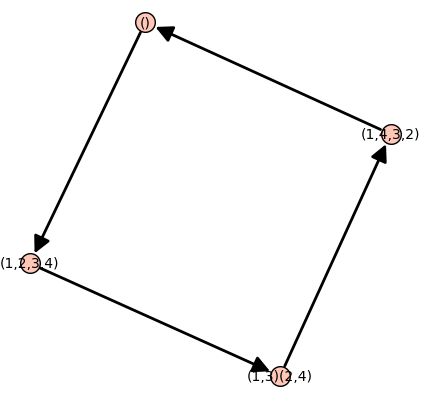
\includegraphics[scale=0.5]{q91.png}
        \captionof{figure}{Graphe de Cayley du groupe $(\mathbb{Z}/4\mathbb{Z}, +, 0)$}
    \end{center}

    \begin{center}
        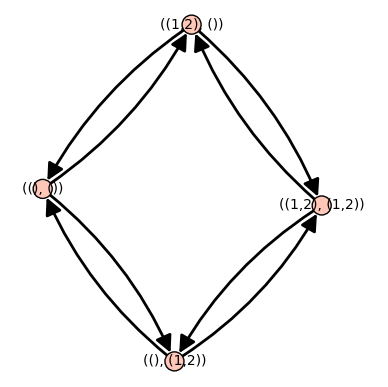
\includegraphics[scale=0.5]{q92.png}
        \captionof{figure}{Graphe de Cayley du groupe $(\mathbb{Z}/2\mathbb{Z}\times\mathbb{Z}/2\mathbb{Z}, +, 0)$}
    \end{center}

    \textbf{Question 10 :}

    \begin{tabularx}{11.5cm}{|p{0.60cm}|X|}
        \hline
        \verb|In|
        & 
        \verb|NOT_CNOT = PermutationGroup(['(1, 3)(2, 4)', '(3, 4)'])|
        \\
        \hline
    \end{tabularx}\newline
    \begin{tabularx}{11.5cm}{|p{0.60cm}|X|}
        \hline
        \verb|In|
        & 
        \verb|NOT_CNOT.order()|
        \\
        \hline
    \end{tabularx}\newline
    \begin{tabularx}{11.5cm}{|p{0.60cm}|X|}
        \hline
        \verb|Out|
        & 
        \verb|8|
        \\
        \hline
    \end{tabularx}\newline
    
    \begin{tabularx}{11.5cm}{|p{0.60cm}|X|}
        \hline
        \verb|In|
        & 
        \verb|SAWP_CNOT = PermutationGroup(['(2, 3)', '(3, 4)'])|
        \\
        \hline
    \end{tabularx}\newline
    \begin{tabularx}{11.5cm}{|p{0.60cm}|X|}
        \hline
        \verb|In|
        & 
        \verb|SAWP_CNOT.order()|
        \\
        \hline
    \end{tabularx}\newline
    \begin{tabularx}{11.5cm}{|p{0.60cm}|X|}
        \hline
        \verb|Out|
        & 
        \verb|6|
        \\
        \hline
    \end{tabularx}\newline

    \begin{tabularx}{11.5cm}{|p{0.60cm}|X|}
        \hline
        \verb|In|
        & 
        \verb|NOT_SWAP = PermutationGroup(['(1, 3)(2, 4)', '(2, 3)'])|
        \\
        \hline
    \end{tabularx}\newline
    \begin{tabularx}{11.5cm}{|p{0.60cm}|X|}
        \hline
        \verb|In|
        & 
        \verb|NOT_SWAP.order()|
        \\
        \hline
    \end{tabularx}\newline
    \begin{tabularx}{11.5cm}{|p{0.60cm}|X|}
        \hline
        \verb|Out|
        & 
        \verb|8|
        \\
        \hline
    \end{tabularx}\newline

    \begin{tabularx}{11.5cm}{|p{0.60cm}|X|}
        \hline
        \verb|In|
        & 
        \verb|NOT_CNOT_SWAP = PermutationGroup(['(1, 3)(2, 4)',|
        \\
        \verb||
        &
        \verb|'(3, 4)','(2, 3)'])|
        \\
        \hline
    \end{tabularx}\newline
    \begin{tabularx}{11.5cm}{|p{0.60cm}|X|}
        \hline
        \verb|In|
        & 
        \verb|NOT_CNOT_SWAP.order()|
        \\
        \hline
    \end{tabularx}\newline
    \begin{tabularx}{11.5cm}{|p{0.60cm}|X|}
        \hline
        \verb|Out|
        & 
        \verb|24|
        \\
        \hline
    \end{tabularx}\newline

    \begin{center}
        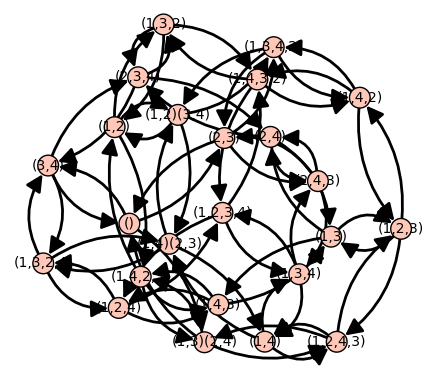
\includegraphics[scale=0.5]{q10.png}
        \captionof{figure}{Graphe de Cayley de $\mathfrak{S}4$ pour le système de générateurs $\{NOT;CNOT;SWAP\}$}
    \end{center}

    \begin{tabularx}{11.5cm}{|p{0.60cm}|X|}
        \hline
        \verb|In|
        & 
        \verb|NOT_CNOT_SWAP.cayley_graph().is_planar()|
        \\
        \hline
    \end{tabularx}\newline
    \begin{tabularx}{11.5cm}{|p{0.60cm}|X|}
        \hline
        \verb|out|
        & 
        \verb|False|
        \\
        \hline
    \end{tabularx}\newline

    En effet, ce graphe possède 24 noeuds. D'après la formule d'Euler, il doit contenir au plus $3*24-6$ arrêtes soit 66 arrêtes. Or ce dernier en contient 72. Il ne peut donc pas être planaire.


\end{document}
